\documentclass[english,xcolor=pst,11pt]{beamer}

%\usetheme{Rochester}
%\usetheme{Berkeley}
\usetheme{Berlin}
\usepackage{beamerthemesplit}


\usepackage[utf8]{inputenc}
\usepackage{amsmath, amssymb, bbm}
\usepackage{url}
\usepackage{hyperref}
\usepackage{physics, slashed}
\usepackage{graphicx}
\usepackage{hyperref}
\usepackage{placeins}
\usepackage{calc}
\usepackage{float}
\usepackage{xcolor}
%\usepackage{accents}
\usepackage{stackrel}
\usepackage{mathtools}
\usepackage{graphicx}
\usepackage{adjustbox}

\usepackage{tikz}
\usetikzlibrary{patterns,math,calc}
\usetikzlibrary{decorations.pathreplacing}
\usetikzlibrary{positioning}
\usetikzlibrary{decorations.pathmorphing}
\usetikzlibrary{decorations.markings}
\usetikzlibrary{arrows}
\renewcommand\epsilon\varepsilon % its probably not consistent in the tex code
\renewcommand\nabla\partial % its probably not consistent in the tex code



\title{Continuous Performance Monitoring of the Grid library on a Supercomputer}
\author{\textbf{Simon Bürger}, Antonin Portelli}
\date{August 8th, 2024}

% \pdfinfo{
%   /Title    (Scattering in Lattice Systems)
%   /Author   (Simon Bürger)
% }

\newlength\leftsidebar
\newlength\rightsidebar
\makeatletter
\setlength\leftsidebar{\beamer@leftsidebar}
\setlength\rightsidebar{\beamer@rightsidebar}
\makeatother

\begin{document}

%\maketitle

\begin{frame}
 \titlepage

\begin{tikzpicture}[remember picture, overlay]
    % Position the logos using node coordinates
    \node[anchor=south west, yshift=1.5cm, xshift=2cm] at (current page.south west) {
\includegraphics[width=2.3cm]{logos/dirac.png}};
    \node[anchor=south west, yshift=3cm, xshift=2cm] at (current page.south west) {
\includegraphics[width=2.3cm]{logos/stfc.png}};

    \node[anchor=south east, yshift=1.5cm, xshift=-2cm] at (current page.south east) {
\includegraphics[width=2.3cm]{logos/epcc.pdf}};
    \node[anchor=south east, yshift=3cm, xshift=-2cm] at (current page.south east) {
\includegraphics[width=2.3cm]{logos/edinburgh.pdf}};

  \end{tikzpicture}
\end{frame}

% \begin{frame}
%  \begin{block}{Overview}
%   \begin{enumerate}
%    \item Goals
%    \item Implementation using TeamCity
%    \item Performance monitoring
%   \end{enumerate}
%  \end{block}
%
% \end{frame}



\section{Motivation and Goals}

\begin{frame}

\textbf{Goals}
\begin{itemize}
 \item \textbf{Continuous integration}: Notice breaking changes as soon as possible, avoid infamous ``works on my machine''
 \item \textbf{Automatic deployment}: Improved reproducibility and simplified user experience
 \item \textbf{Performance monitoring}: Detect performance regressions, caused by any part of the system
\end{itemize}

\end{frame}

\begin{frame}

\section{TeamCity Implementation}
\textbf{Jetbrains TeamCity Architecture}
\begin{figure}[H]
	\centering
  %\input{plots/schemes/schemes_quenched}
  %\adjustbox{trim={.01\width} {.35\height} {0.01\width} {.35\height},clip}%
    {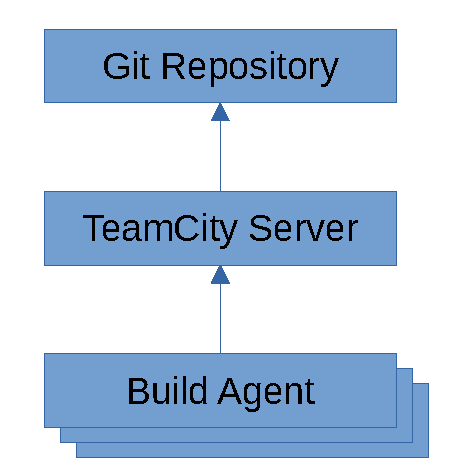
\includegraphics[width=1.8in]{diagrams/teamcity.pdf}}
\end{figure}
\vfill
\begin{itemize}
 \item Scalable to arbitrary number of build servers
 \item Communication via https
\end{itemize}




\end{frame}

\begin{frame}
\textbf{Dedicated CICD hardware}
 \begin{figure}[H]
	\centering
  %\input{plots/schemes/schemes_quenched}
  %\adjustbox{trim={.01\width} {.35\height} {0.01\width} {.35\height},clip}%
    {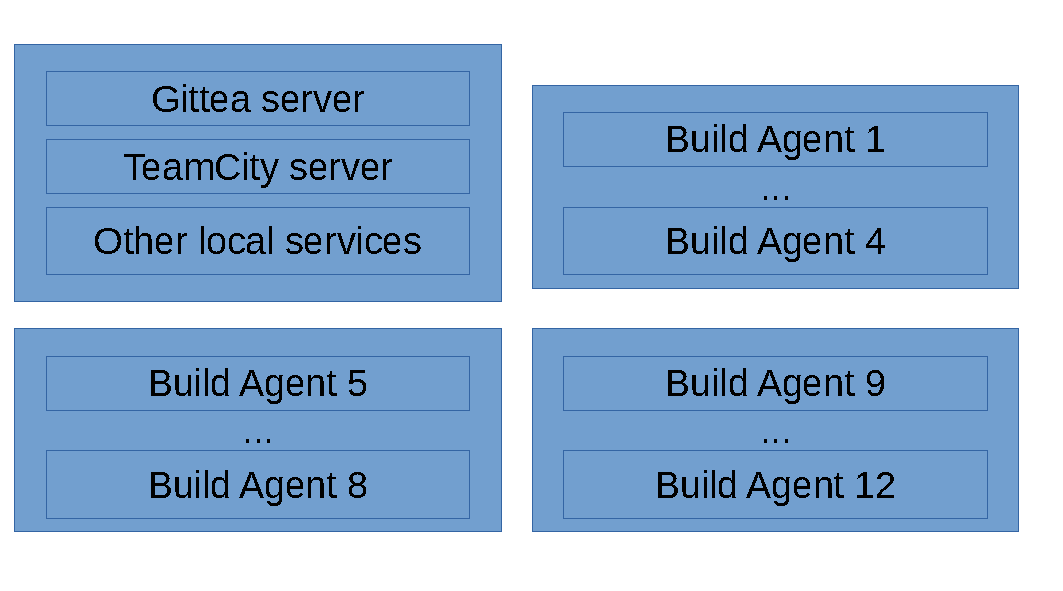
\includegraphics[width=3.2in]{diagrams/hardware.pdf}}
\end{figure}

\begin{itemize}
 \item Four x86 servers, environment identical to the HPC clusters login nodes
 \item Head server runs docker containers of various services, publicly visibly
 \item Agents run on bare metal, not publicly visibly
\end{itemize}

\end{frame}

\begin{frame}
 \textbf{Triggers for the CI system}
\begin{itemize}
 \item Each commit, including pending pull requests \\$\longrightarrow$ Build Grid and Hadrons and run unittests
 \item Once per day: \\$\longrightarrow$ deploy new production binaries if there were any changes \\
 $\longrightarrow$ run benchmarks, using latest production binaries
 \item Benchmarking is run regardless of source code changes, thus effectively monitors the runtime environment as well.
\end{itemize}
\end{frame}

\section{HPC cluster integration}
\begin{frame}
 \textbf{Integration into the HPC cluster \emph{Tursa}}
 \begin{itemize}
  \item Problem: Build servers do not have GPUs
  \item Solution: GPU-based unittests and benchmarking jobs are submitted via SLURM to the computing cluster
  \item Finished jobs report back to TeamCity via a REST API
 \end{itemize}

\end{frame}

\section{Showcase}
\begin{frame}
 \textbf{What does it look like?}\\
 On a GitHub pull request:
  \begin{figure}[H]
	\centering
  %\input{plots/schemes/schemes_quenched}
  %\adjustbox{trim={.01\width} {.35\height} {0.01\width} {.35\height},clip}%
    {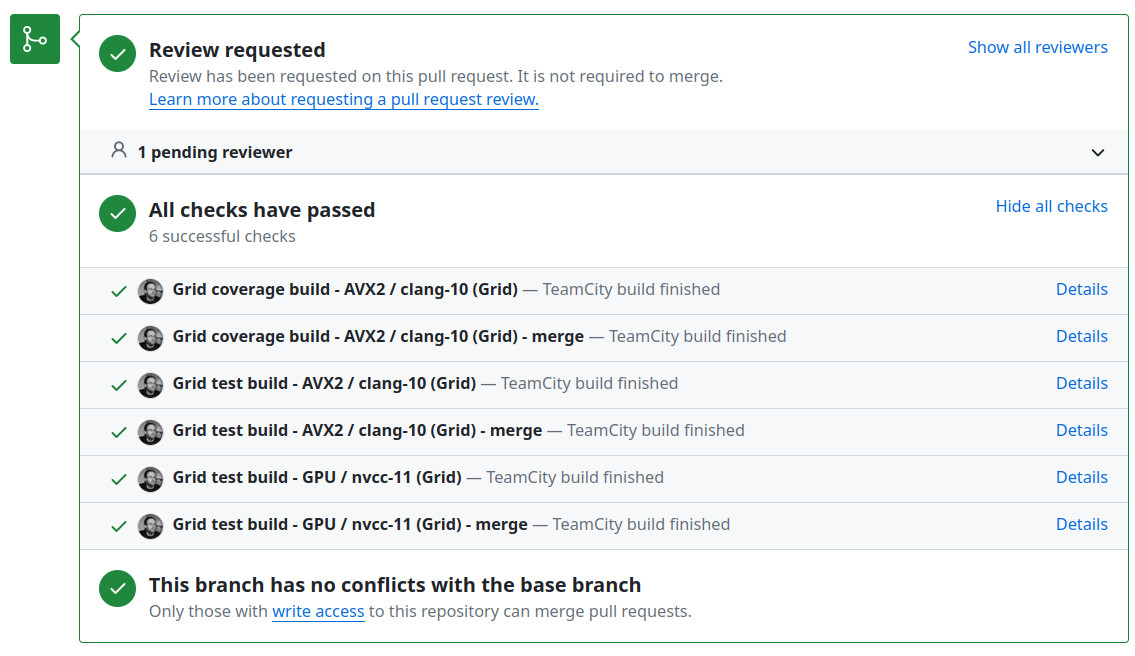
\includegraphics[width=4.5in]{diagrams/pr.jpg}}
\end{figure}
\end{frame}


{ % all template changes are local to this group.
    \setbeamertemplate{navigation symbols}{}
    \begin{frame}<article:0>[plain]
        \begin{tikzpicture}[remember picture,overlay]
            \node[at=(current page.center)] {
                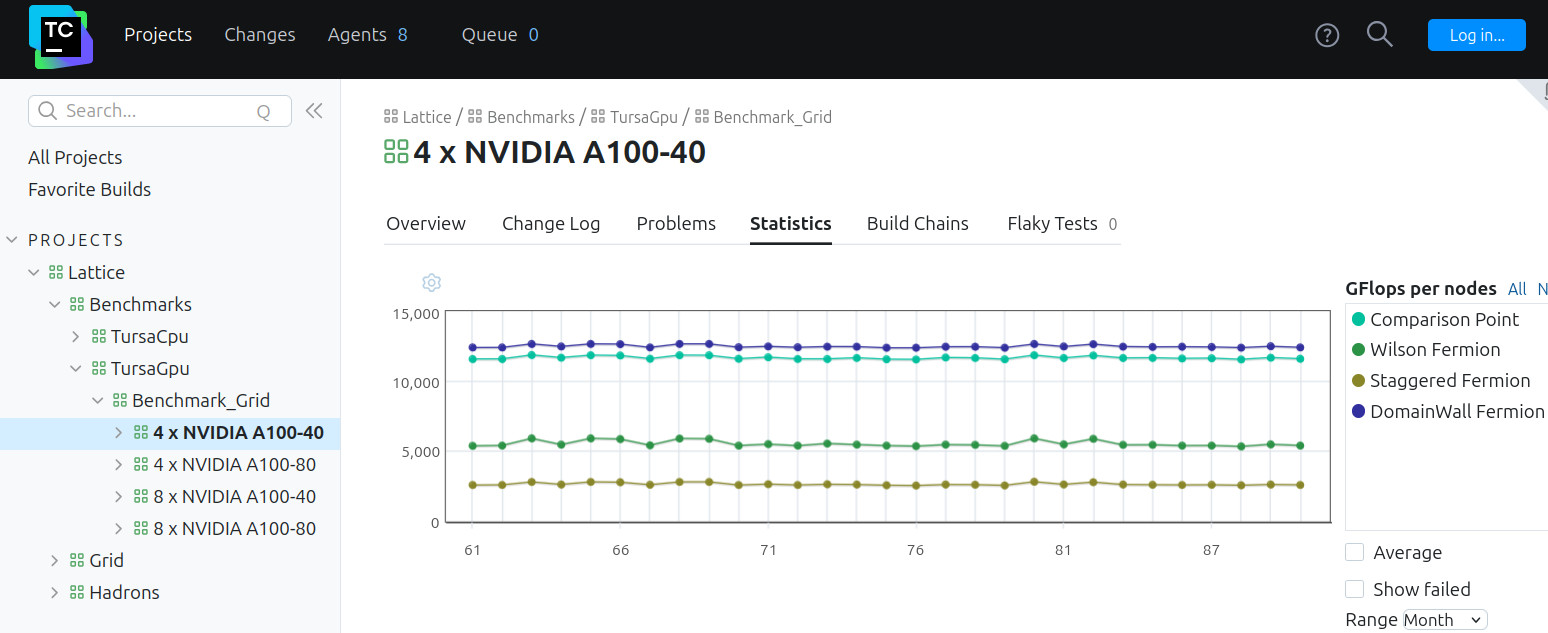
\includegraphics[keepaspectratio,
                                 width=\paperwidth,
                                 height=\paperheight]{diagrams/benchmarks.jpg}
            };
        \end{tikzpicture}
     \end{frame}
}

\section{Discussion}
\begin{frame}
 \textbf{Stability}
 \begin{itemize}
  \item All build artifacts are backed up to a cloud storage provider
  \item Configuration of TeamCity itself is tracked in a git repository
  \end{itemize}
  \textbf{Hardening}
  \begin{itemize}
  \item Build servers are not publicly visible, communication to main server is ``one-way''
  \item Build agents run as dedicated  user with limited permissions on the cluster, e.g., no access to research data
 \end{itemize}
 \textbf{Future outlook}

 \begin{itemize}
  \item Solution is scalable to multiple HPC clusters
 \end{itemize}
TODO: This CI/CD solution was funded by the STFC DiRAC Facility
\end{frame}


\begin{frame}
 \Large{\textbf{Questions?}} \\ \vfill
 \small{(for a live demo, come talk to me later. TODO: link)}
\end{frame}




\end{document}
